%!TEX root = main.tex
\section{Análisis exploratorio de datos}

El \href{https://www.ibm.com/es-es/cloud/learn/exploratory-data-analysis}{análisis exploratorio de datos} es un proceso que permite conocer a priori la naturaleza de los conjuntos.

El análisis exploratorio de datos (AED) es una etapa crucial en la investigación y el análisis de datos. Su objetivo es comprender la estructura y las características de un conjunto de datos antes de aplicar técnicas estadísticas más avanzadas o construir modelos predictivos. El AED ayuda a identificar patrones, tendencias, valores atípicos y relaciones entre variables, lo que permite formular hipótesis y generar conocimientos preliminares sobre los datos, respondiendo así algunas preguntas como: 

\begin{enumerate}
    \item ¿Cuál es la distribución de las variables en el conjunto de datos?
    \item ¿Existen correlaciones entre las variables?
    \item ¿Hay valores atípicos que necesiten ser investigados?
    \item ¿Cuáles son las características más relevantes o distintivas del conjunto de datos?
    \item ¿Hay patrones o tendencias interesantes que se puedan identificar?
\end{enumerate}

En particular en esta ocasión nos permite obtener algunas posibles conclusiones:

\begin{enumerate}
    \item \textbf{Patrones temporales:} Al analizar los datos a lo largo del período de tiempo (del 1 de marzo de 2013 al 28 de febrero de 2017), es posible identificar patrones temporales en la contaminación del aire. Esto puede revelar estacionalidades, tendencias a largo plazo y variaciones interanuales en la calidad del aire en Beijing.
    \item \textbf{Variaciones geográficas:} Al tener datos de 12 sitios de monitoreo de calidad del aire en Beijing, es posible analizar las variaciones geográficas en los niveles de contaminantes. Esto puede revelar áreas específicas que son más susceptibles a altos niveles de contaminación o identificar diferencias significativas en la calidad del aire entre diferentes partes de la ciudad.
    \item \textbf{Correlaciones entre contaminantes:} Al analizar los datos de los cinco contaminantes atmosféricos (SO2, NO2, PM10, CO y O3), se pueden identificar correlaciones y relaciones entre ellos. Por ejemplo, es posible que se encuentre una correlación positiva entre los niveles de NO2 y PM10, lo que sugiere que ciertos contaminantes están relacionados entre sí.
    \item \textbf{Influencia de los factores meteorológicos:} Al relacionar los datos de calidad del aire con los datos meteorológicos de la estación más cercana, se puede investigar la influencia de los factores meteorológicos en la contaminación del aire. Esto puede revelar cómo variables como la temperatura, la humedad, la velocidad del viento, etc, pueden afectar los niveles de contaminantes y proporcionar información útil para comprender los factores que contribuyen a la calidad del aire en Beijing.
    \item \textbf{Interpretación del Índice de Calidad del Aire (AQI):} Al comprender cómo se calcula y se interpreta el Índice de Calidad del Aire (AQI) en función de los cinco contaminantes atmosféricos mencionados (SO2, NO2, PM10, CO y O3), se puede proporcionar una interpretación más detallada y precisa de la calidad del aire en diferentes días y contextos.
\end{enumerate}

El objetivo es obtener una comprensión más profunda de la calidad del aire en Beijing, identificar patrones y relaciones clave, y proporcionar información útil para futuras investigaciones y medidas de control de la contaminación o en el desarrollo de modelos.\cite{liang2016spatiotemporal}

\begin{figure}[htb] 
    \begin{center} 
        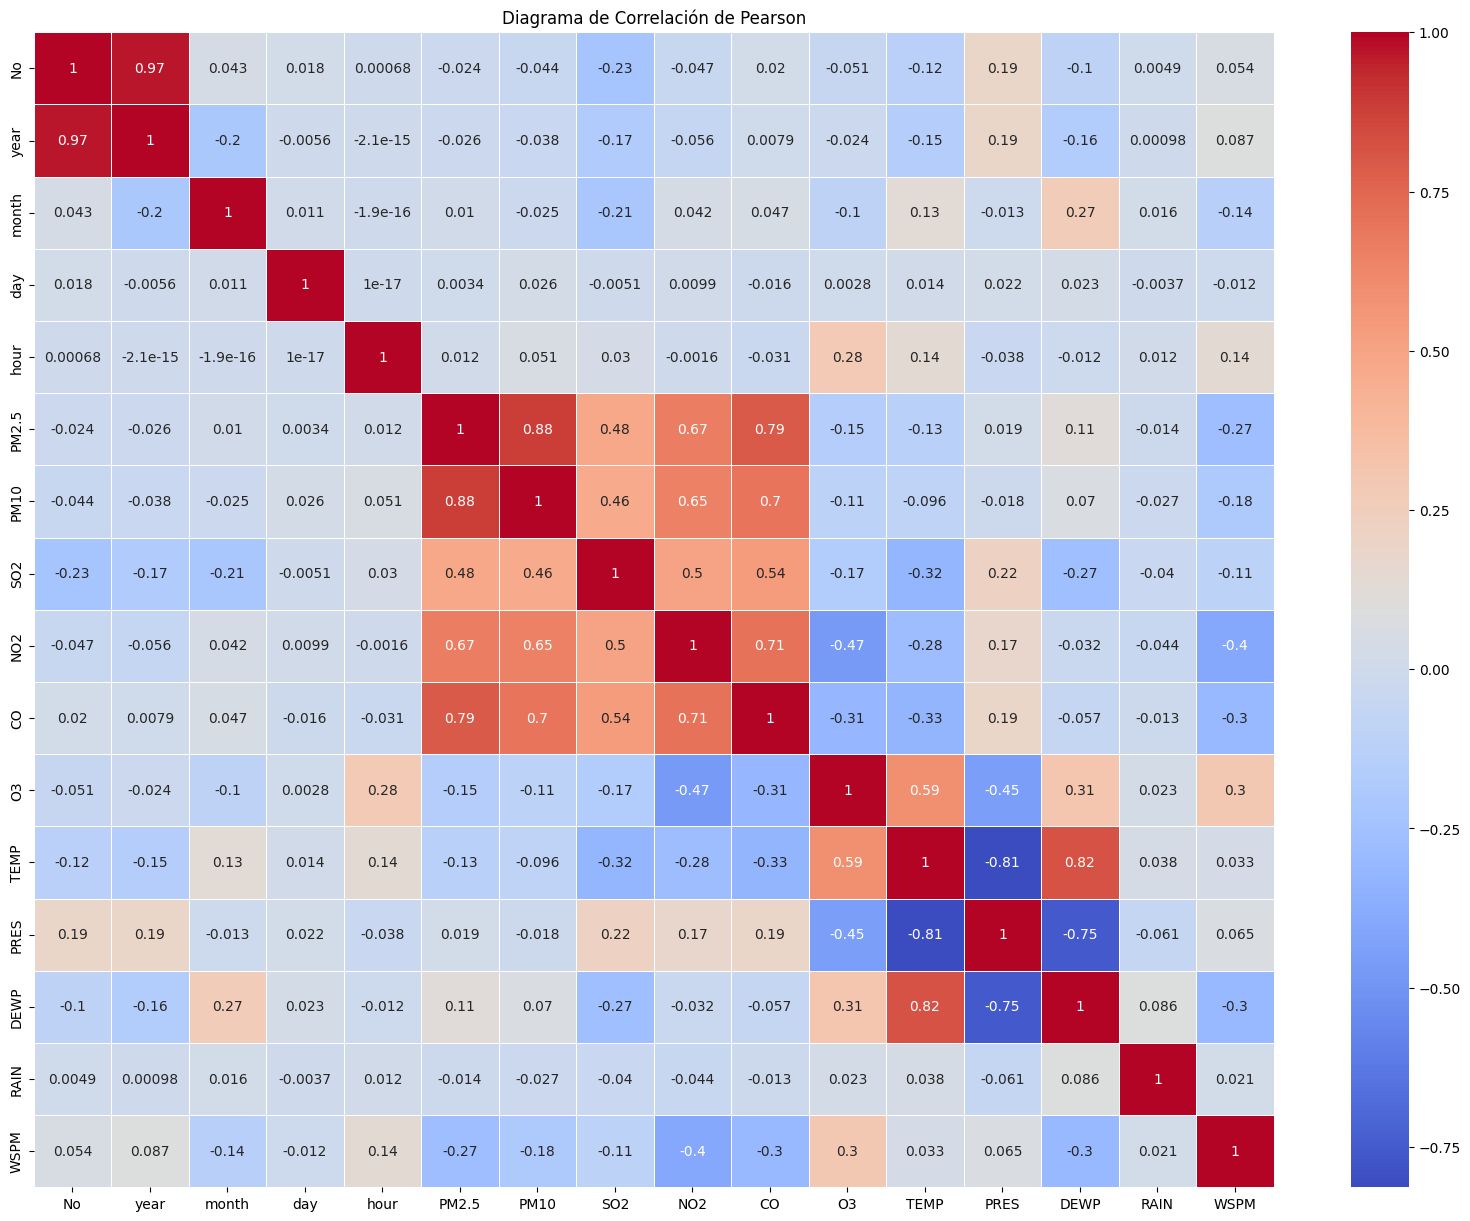
\includegraphics[width=8cm]{Papper IB/Images/correlation_matrix.png}
    \end{center} 
    \caption{Matriz de Correlación de Pearson.} 
    \label{fig:fig1} 
\end{figure} 

Informe: Análisis de correlaciones en el conjunto de datos de calidad del aire de Beijing

La matriz de correlación de Pearson se usa con el objetivo de comprender las correlaciones entre las variables y proporcionar una visión más profunda de la contaminación del aire en Beijing, se presentan los hallazgos clave derivados del análisis de correlaciones.

\subsection{\textbf{Correlación positiva fuerte}}
Se observó una correlación positiva fuerte (0.884380) entre los niveles de partículas suspendidas de diámetro menor a 2.5 micrómetros (PM2.5) y los niveles de partículas suspendidas de diámetro menor a 10 micrómetros (PM10). Esta correlación indica que los niveles de partículas PM2.5 están altamente correlacionados con los niveles de partículas PM10. Es importante tener en cuenta que las partículas PM2.5 son un subconjunto de las partículas PM10.

\subsection{\textbf{Correlaciones positivas moderadas}}
Se encontraron correlaciones positivas moderadas entre los niveles de partículas PM2.5 y los niveles de monóxido de carbono (CO) (0.789998) y dióxido de nitrógeno (NO2) (0.666948). Estas correlaciones sugieren que los niveles de partículas suspendidas de diámetro menor a 2.5 micrómetros están relacionados con la presencia de CO y NO2 en el aire. Esto indica que la presencia de CO y NO2 puede contribuir a la contaminación del aire por partículas PM2.5.

\subsection{\textbf{Correlación negativa moderada}}
Se encontró una correlación negativa moderada (-0.349856) entre los niveles de dióxido de azufre (SO2) y los niveles de dióxido de nitrógeno (NO2). Esta correlación inversa indica que los niveles de SO2 y NO2 en el aire tienden a tener una relación inversa. Es importante considerar esta relación en el contexto de la calidad del aire, ya que la presencia de estos contaminantes puede tener diferentes fuentes y efectos en la salud y el medio ambiente.

\subsection{\textbf{Correlación con variables meteorológicas}}
Se observaron correlaciones débiles a moderadas entre las variables de contaminantes atmosféricos (PM2.5, PM10, SO2, NO2, CO, O3) y las variables meteorológicas (TEMP, PRES, DEWP, RAIN, WSPM). Estas correlaciones indican que los factores meteorológicos pueden influir en los niveles de contaminantes en el aire. Por ejemplo, la temperatura (TEMP) puede estar relacionada con la formación de ozono (O3), y la velocidad del viento (WSPM) puede afectar la dispersión de los contaminantes. Sin embargo, es importante destacar que estas correlaciones son de naturaleza débil a moderada y se requiere un análisis más profundo para comprender plenamente la influencia de los factores meteorológicos en la contaminación del aire.

En conclusión, el análisis de correlaciones ha proporcionado información valiosa sobre las relaciones entre las variables. Estas correlaciones destacan la fuerte relación entre las partículas PM2.5 y PM10, así como las asociaciones moderadas entre los contaminantes atmosféricos y los factores meteorológicos. Estos hallazgos contribuyen a una mejor comprensión de los factores y pueden servir como base para investigaciones posteriores y medidas de control de la contaminación atmosférica en la región.\cite{liang2017comparison}

\subsection{\textbf{Simetría de los datos}}
Se analizó la diferencia entre la media y la mediana de las variables numéricas en el conjunto de datos, con el fin de obtener información sobre la simetría de la distribución de los datos y la presencia de valores atípicos. 

\begin{itemize}
    \item \textbf{Diferencias nulas:} Se observó que las variables "No" y "hour" presentan una diferencia de cero entre la media y la mediana. Esto indica que no hay una discrepancia significativa entre estos valores estadísticos para dichas variables. En otras palabras, la distribución de los datos para estas variables es simétrica.
    \item \textbf{Diferencias negativas:} Las variables "year", "month", "day", "TEMP" y "DEWP" mostraron diferencias negativas entre la media y la mediana. Estas diferencias sugieren que estas variables tienden a tener una distribución asimétrica hacia la izquierda. Es decir, la concentración de valores más bajos arrastra la media hacia abajo en comparación con la mediana.
    \item \textbf{Diferencias positivas:} Por otro lado, se encontró que las variables "PM2.5", "PM10", "SO2", "NO2", "CO", "O3", "PRES", "RAIN" y "WSPM" presentaron diferencias positivas entre la media y la mediana. Esto indica que estas variables tienden a tener una distribución asimétrica hacia la derecha. En otras palabras, la presencia de valores más altos influye en la media y la aleja de la mediana.
\end{itemize}

\begin{figure}[htb] 
    \begin{center} 
        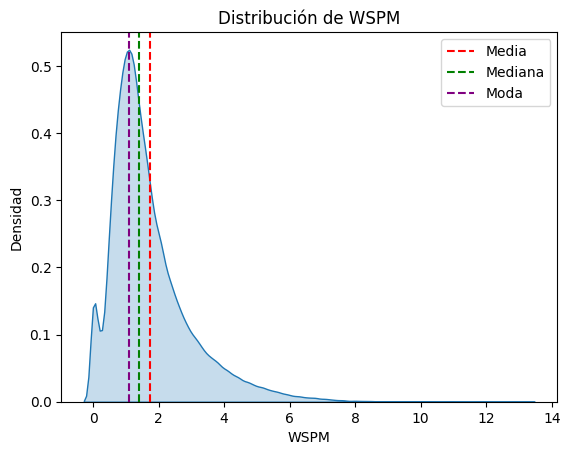
\includegraphics[width=8cm]{Papper IB/Images/simetria_wspm.png}
    \end{center} 
    \caption{Simetría WSPM.} 
    \label{fig:fig1} 
\end{figure} 

Es importante tener en cuenta que estas diferencias entre la media y la mediana son indicadores de la distribución de los datos y pueden sugerir la presencia de valores atípicos o asimetría en los conjuntos de datos correspondientes a cada variable.

\subsection{Tendencias y variaciones}
Obtener gráficos de puntos que representen la mediana de diferentes variables relacionadas con la calidad del aire, como PM2.5, PM10, SO2, NO2, CO, O3, entre otras, en función de los meses y los años.

\begin{figure}[htb] 
    \begin{center} 
        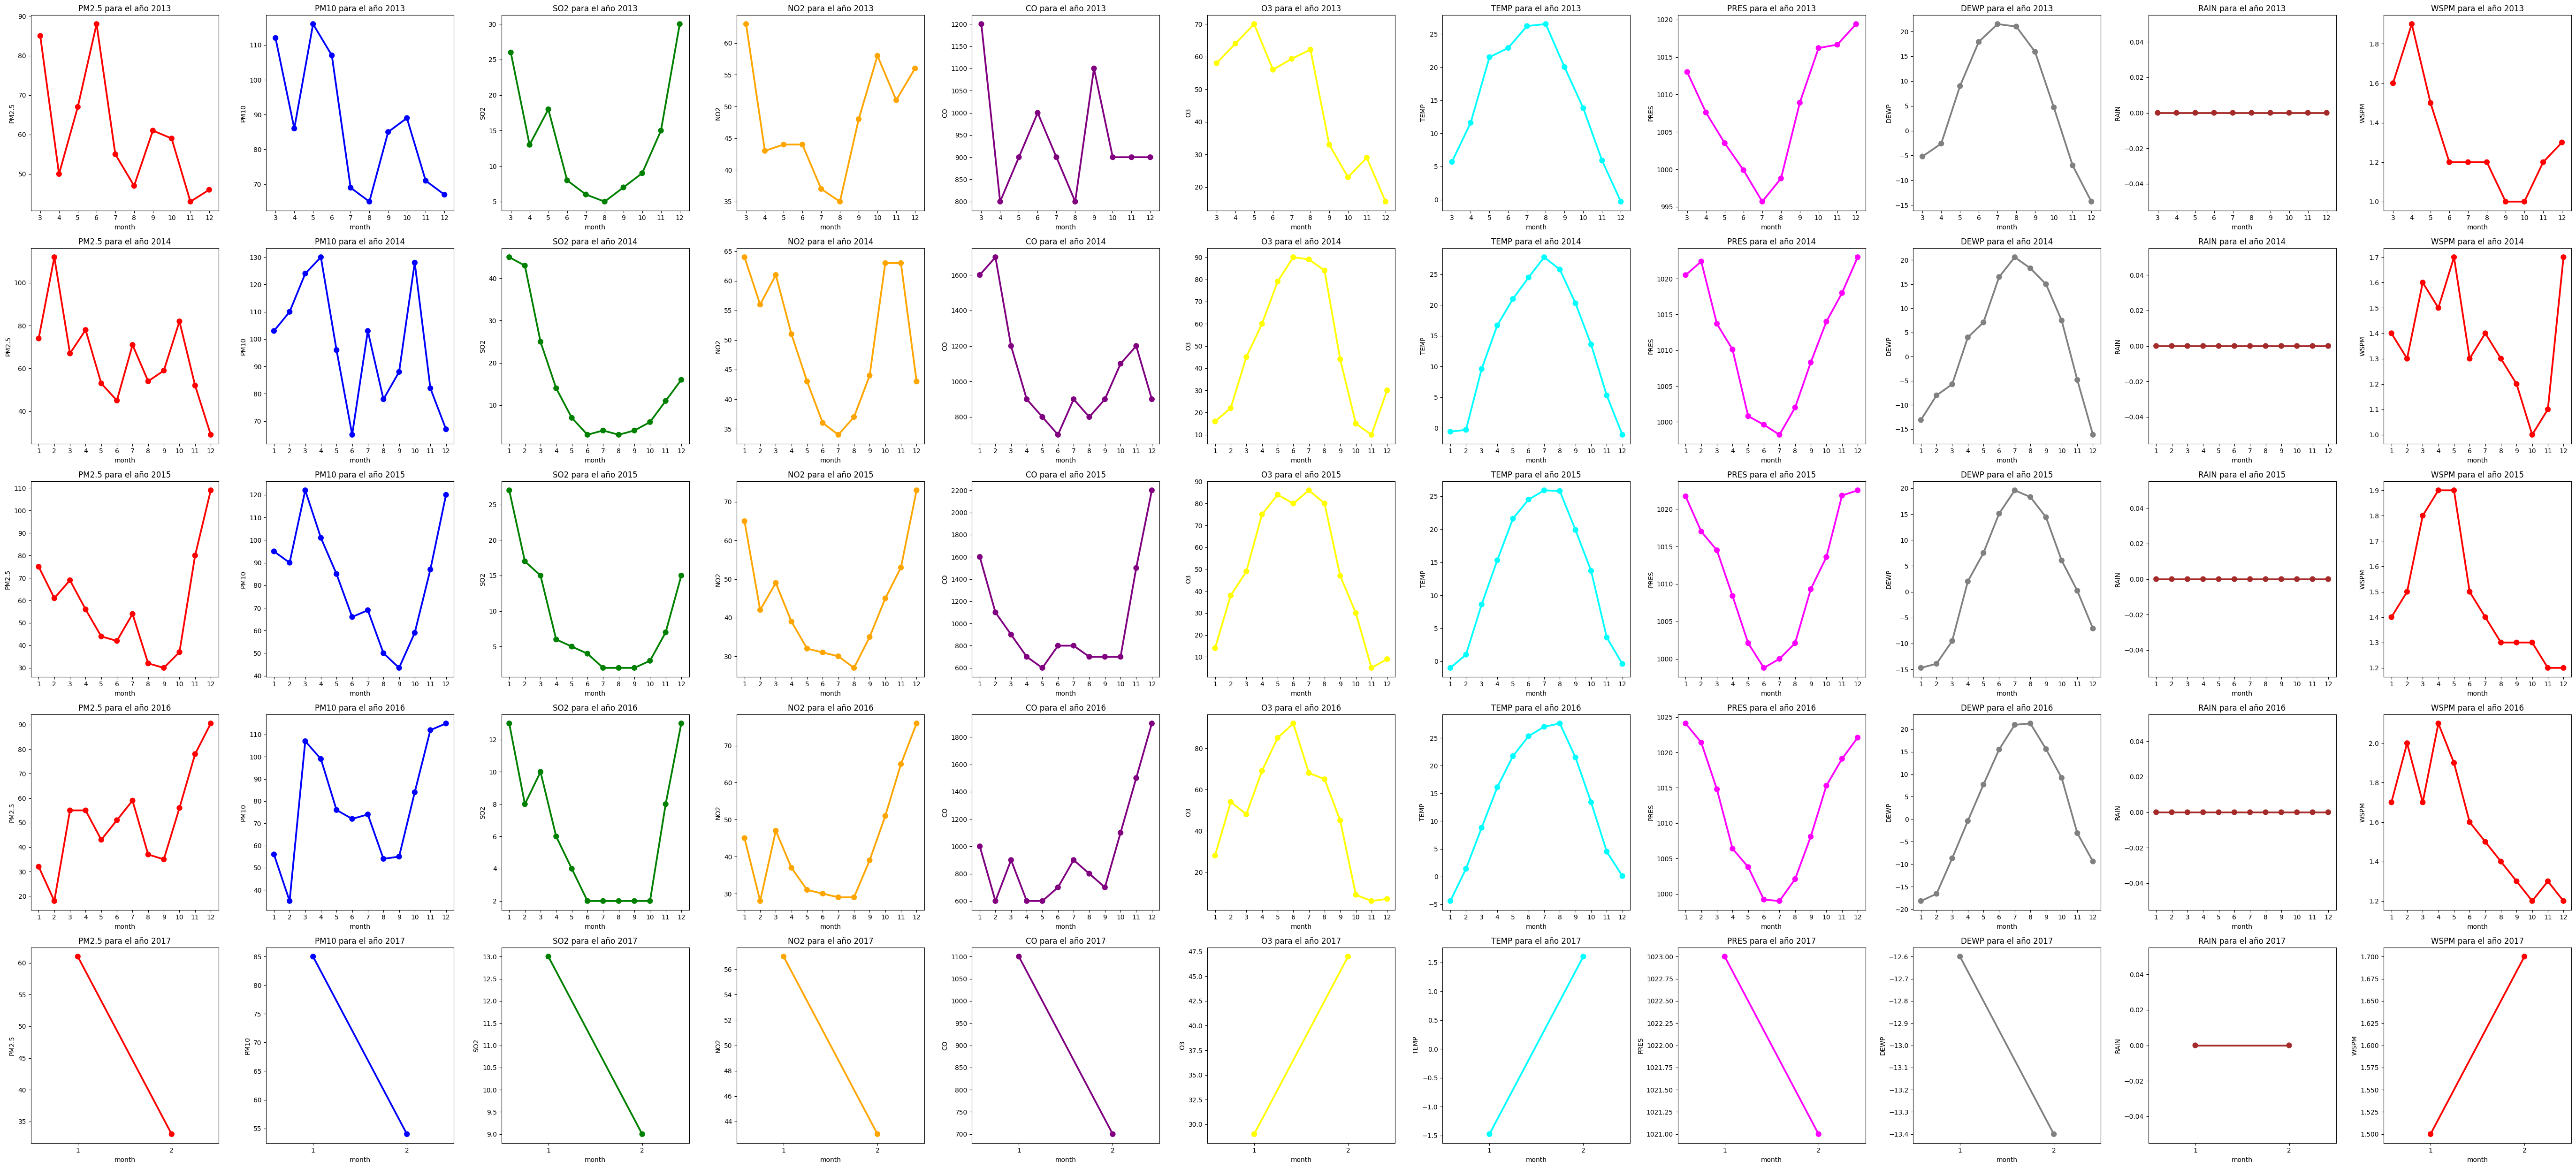
\includegraphics[width=8cm]{Papper IB/Images/expands_all_years.png}
    \end{center} 
    \caption{Simetría WSPM.} 
    \label{fig:fig1} 
\end{figure} 

El análisis permite una exploración visual detallada de la calidad del aire en Beijing a lo largo de los años y los meses. Esto proporcionaría información clave sobre patrones estacionales, cambios a largo plazo y eventos excepcionales en la calidad del aire en la región, lo que sería fundamental para comprender y abordar los desafíos relacionados con la contaminación atmosférica.\cite{liu2018spatio}

El análisis exploratorio de datos es un proceso iterativo, y es posible que nuevas preguntas e hipótesis surjan a medida que se profundiza en los datos y se descubren nuevas perspectivas.